\textbf{See the instruction for questions \inteval{\value{question}+1} to \inteval{\value{question}+3}.}

General instruction (if any) goes here.

\begin{figure}[H]
\centering
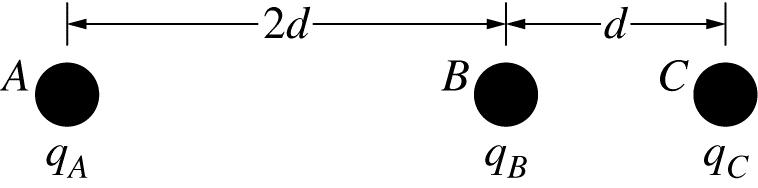
\includegraphics[scale=0.3]{images/img-010-017.png}
\end{figure}

Three small spheres, $A$, $B$, and $C$, have charges with magnitudes $q_{A}$, $q_{B}$, and $q_{C}$, respectively. The three spheres are aligned along a straight line, as shown in the figure above. At the instant shown, the net force on sphere $A$ is zero.

% Multiple Choice Question 20
\begin{questions}\setcounter{question}{19}\question
The ratio $q_{C} / q_{B}$ is

\begin{oneparchoices}
\choice $9 / 4$
\choice $1 / 1$
\choice $4 / 9$
\choice $1 / 4$
\choice $1 / 9$
\end{oneparchoices}\end{questions}

% Multiple Choice Question 21
\begin{questions}\setcounter{question}{20}\question
Which of the following statements must be true of the signs of the charges?

\begin{choices}
\choice Only charges $q_{A}$ and $q_{B}$ have the same sign.
\choice Only charges $q_{A}$ and $q_{C}$ have the same sign.
\choice Only charges $q_{B}$ and $q_{C}$ have the same sign.
\choice Charges $q_{B}$ and $q_{C}$ have different signs.
\choice Charges $q_{A}$, $q_{B}$, and $q_{C}$ all have the same sign.
\end{choices}\end{questions}

% Multiple Choice Question 22
\begin{questions}\setcounter{question}{21}\question
Which of the following is true about the sign of charge $q_{A}$ ?

\begin{choices}
\choice The sign of charge $q_{A}$ must be the same as that of $q_{B}$.
\choice The sign of charge $q_{A}$ must be the same as that of $q_{C}$.
\choice The sign of charge $q_{A}$ must be the same as that of either $q_{B}$ or $q_{C}$, whichever has the greater magnitude.
\choice The sign of charge $q_{A}$ must be the same as that of either $q_{B}$ or $q_{C}$, whichever has the lesser magnitude.
\choice It is possible that $q_{A}$ could be either positive or negative.
\end{choices}\end{questions}

